\section{POD Analysis}
\label{ch:pod}

Open from `3.\ Analysis $\to$ POD Analysis`.

Proper Orthogonal Decomposition (POD) finds the most efficient low-dimensional representation of the velocity field by decomposing the fluctuation field into a set of orthogonal spatial modes $\boldsymbol{\phi}_n(\mathbf{x})$ and corresponding temporal coefficients $a_n(t)$:
\[
\mathbf{u}'(\mathbf{x}, t) = \sum_{n=1}^{N} a_n(t)\,\boldsymbol{\phi}_n(\mathbf{x})
\]
The modes are ordered by their energy content: Mode 1 captures the largest fraction of the total TKE, Mode 2 the next largest, and so on. This property, known as optimality, means that the POD is the most efficient basis for representing the flow in a least-squares sense (Lumley, 1967; Holmes et al., 1996). In practice, a small number of modes often captures the dominant coherent structures (recirculation zones, vortex shedding, shear layer flapping), while the remaining modes represent incoherent noise.

\href{https://cmdrryder.github.io/uPrime/}{uPrime} implements the snapshot POD method (Sirovich, 1987), which is efficient when the number of spatial grid points exceeds the number of snapshots. The SVD of the fluctuation snapshot matrix directly yields the POD modes and their energy content.

\noindent\textbf{References:} Lumley, J.L. (1967). The structure of inhomogeneous turbulent flows. In \textit{Atmospheric Turbulence and Radio Wave Propagation}, 166--178. Holmes, P., Lumley, J.L. \& Berkooz, G. (1996). \textit{Turbulence, Coherent Structures, Dynamical Systems and Symmetry}. Cambridge University Press. Sirovich, L. (1987). Turbulence and the dynamics of coherent structures. \textit{Quarterly of Applied Mathematics}, 45(3), 561--590.

\subsection{Computing POD}

```{note}
\begin{enumerate}[leftmargin=1.5em, topsep=2pt]
  \item Set `Modes to compute` (default 25). Increasing this takes longer.
  \item Click `Compute POD`. For large datasets this may take several seconds to a minute.
  \item All four tabs populate automatically when done.
\end{enumerate}
```

```{note}
POD uses all velocity components simultaneously (U+V for 2D2C; U+V+W for 2D3C). The energy percentage of each mode reflects the combined energy across all components.
```

\subsection{Energy Spectrum tab}

Use the energy spectrum to decide how many modes to use for reconstruction and interpretation. A steep drop after Mode 1 or 2 indicates a flow dominated by one or two strong coherent structures. A slow gradual decay indicates broadband turbulence with energy distributed across many scales.

\begin{figure}[htbp]
  \centering
  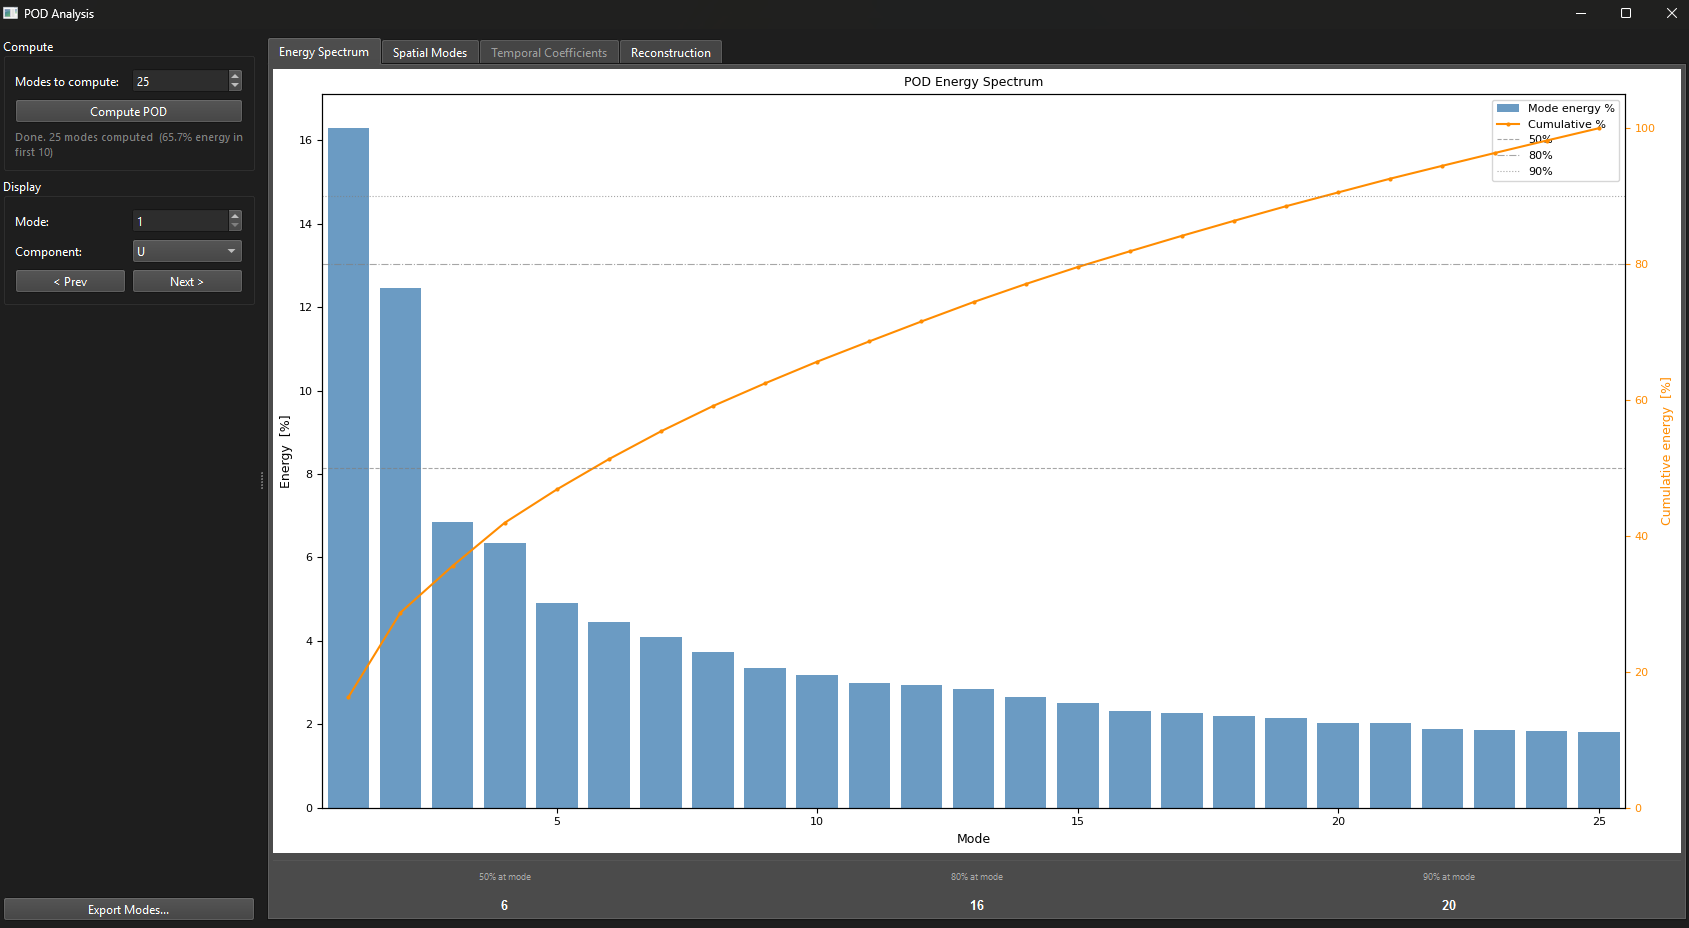
\includegraphics[width=0.92\linewidth]{fig8}
  \caption{POD Energy Spectrum tab. Bars show the energy percentage per mode; the orange curve shows cumulative energy. Dashed horizontal lines mark the 50\%, 80\%, and 90\% thresholds. The readout strip at the bottom shows how many modes are needed to reach each threshold.}
  \label{fig:pod_energy}
\end{figure}

\subsection{Spatial Modes tab}

Use the `Mode` spinbox or `$<$ Prev` / `Next $>$` buttons to step through modes. Use the `Component` dropdown to inspect different velocity directions. The title shows the mode number and its energy fraction.

\begin{figure}[htbp]
  \centering
  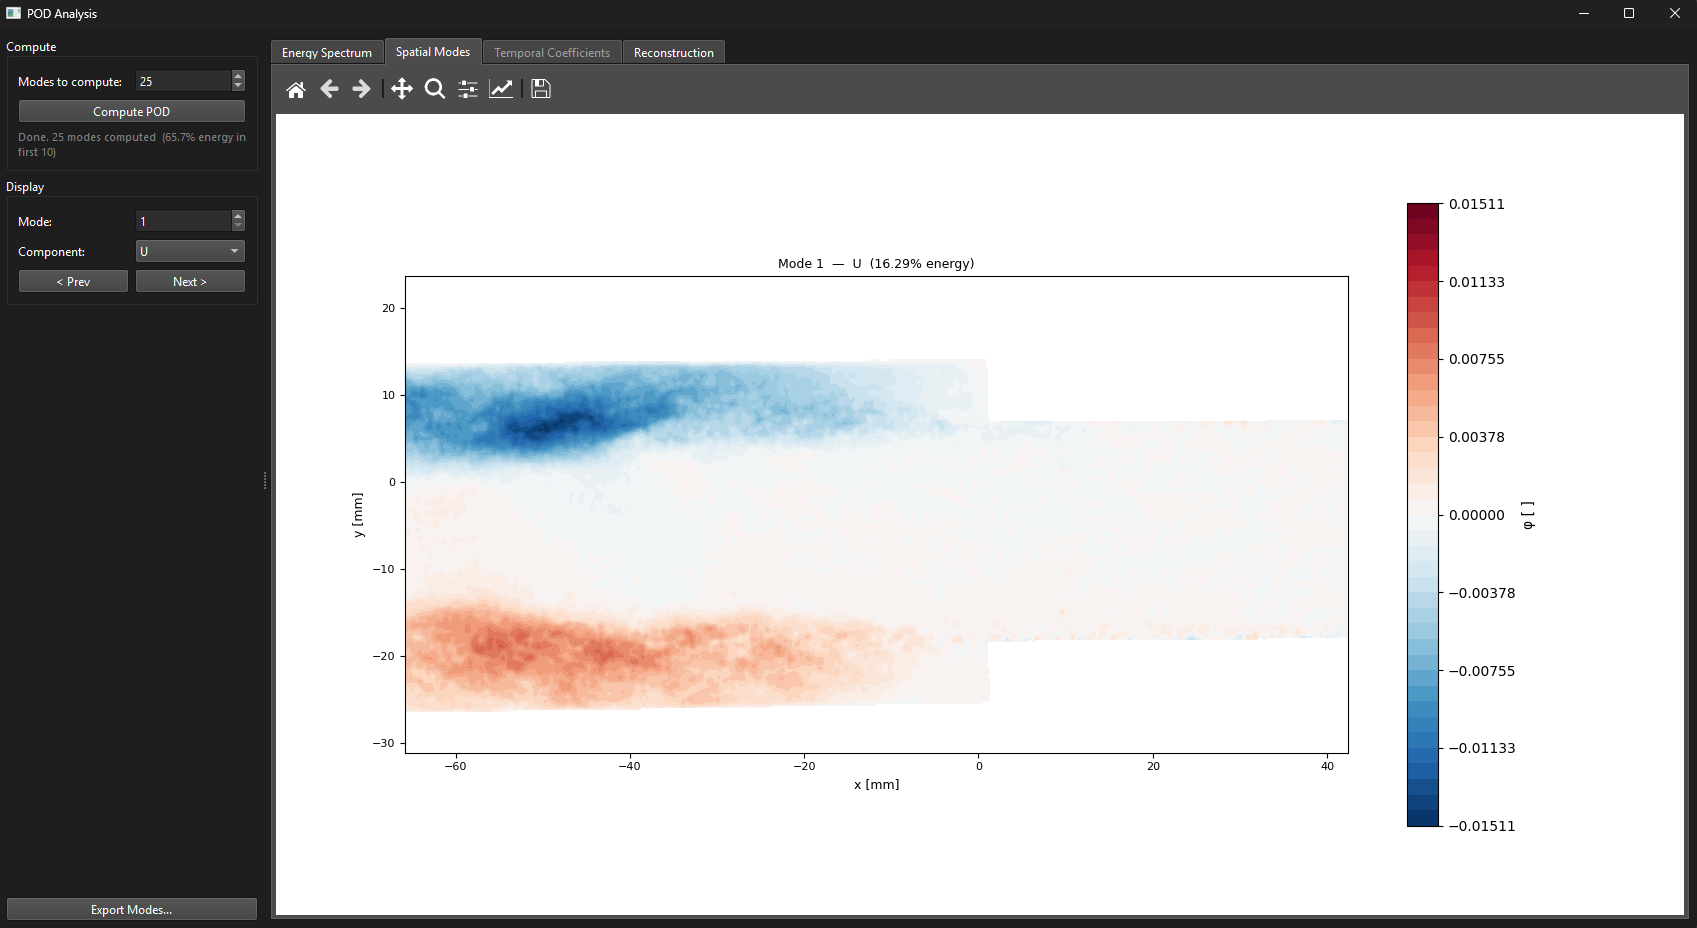
\includegraphics[width=0.92\linewidth]{fig9}
  \caption{POD Spatial Modes tab showing Mode~1 of the $U$ component. Red and blue regions represent opposite-signed velocity fluctuations associated with the dominant coherent structure in the flow. The energy fraction of the mode is shown in the plot title.}
  \label{fig:pod_mode}
\end{figure}

\subsection{Temporal Coefficients tab (TR only)}

Shows the temporal coefficient time series $a_n(t)$ for the selected mode and its power spectral density. A sharp peak in the PSD indicates a periodic structure at that frequency (e.g.\ vortex shedding or shear layer flapping).

\subsection{Reconstruction tab}

\begin{figure}[htbp]
  \centering
  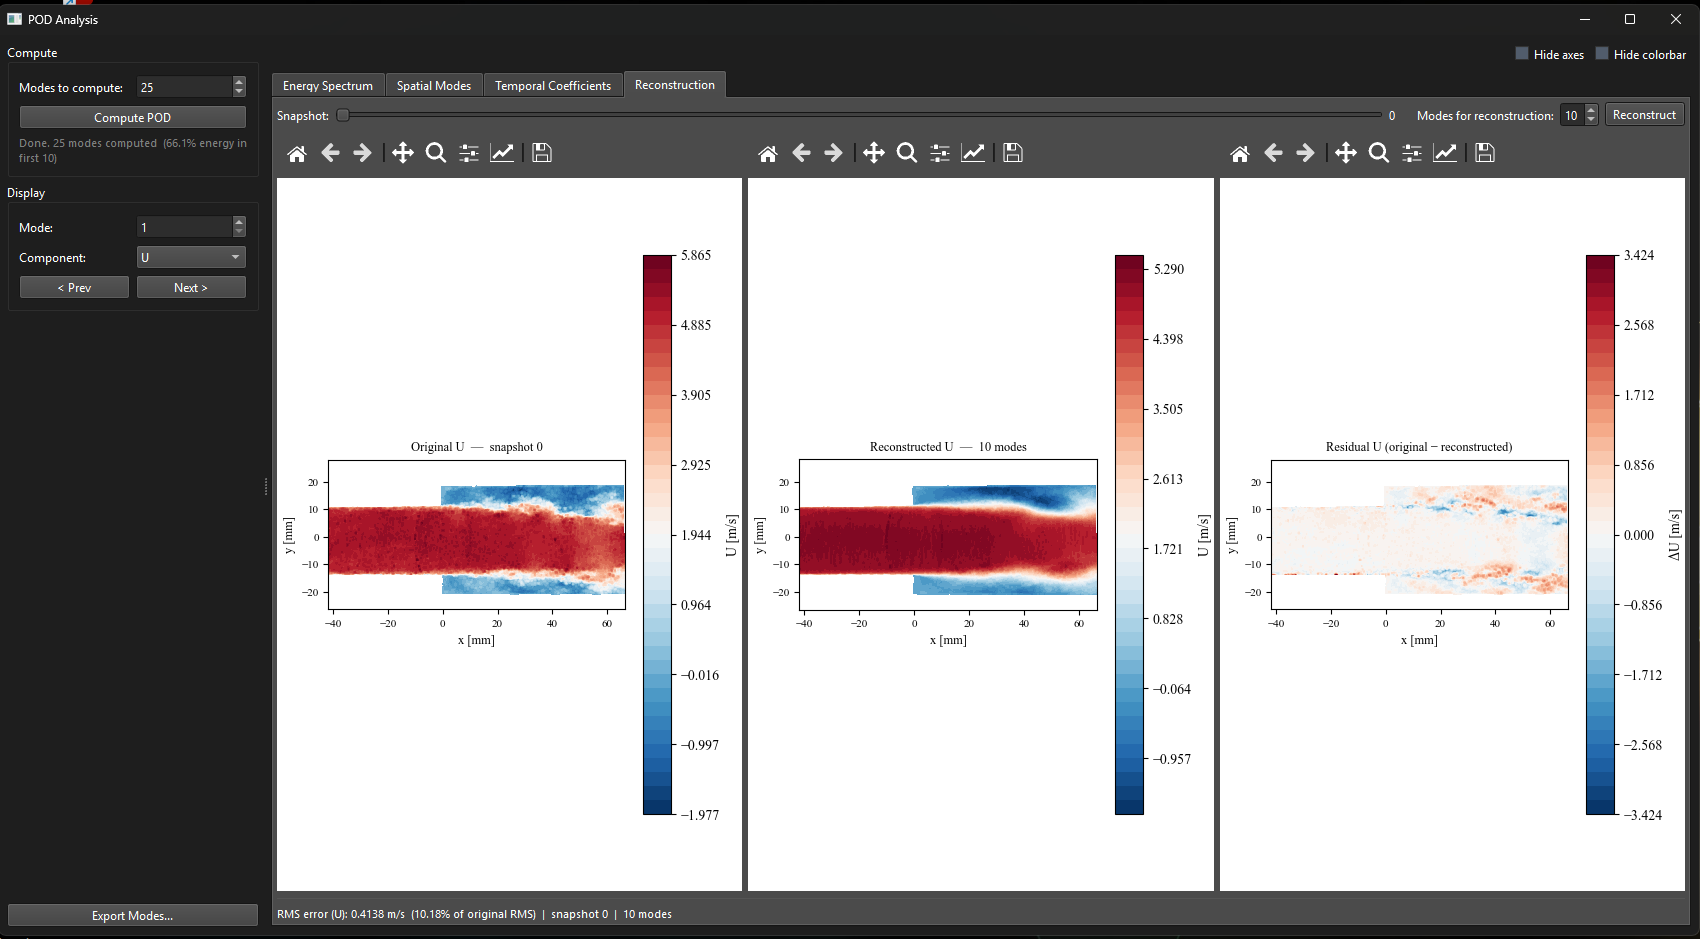
\includegraphics[width=0.92\linewidth]{fig10}
  \caption{POD Reconstruction tab. Left: original snapshot. Center: low-order reconstruction with selected modes. Right: residual (original minus reconstructed). The RMS reconstruction error is shown at the bottom.}
  \label{fig:pod_recon}
\end{figure}

```{note}
\begin{enumerate}[leftmargin=1.5em, topsep=2pt]
  \item Drag the `Snapshot` slider to select a snapshot.
  \item Set `Modes for reconstruction` (minimum 1).
  \item Click `Reconstruct`.
\end{enumerate}
```

The three panels show the original field, the low-order reconstruction, and the residual. A residual below 10--20\% RMS generally means the selected modes capture the dominant structure.

\subsection{Exporting}

Click `Export Modes\ldots` to save all spatial modes as a Tecplot \texttt{.dat} file and temporal coefficients as a \texttt{.csv} file.

% ============================= CHAPTER 11 ==============================
